\documentclass[11pt, a4 paper]{article}


\usepackage{/Users/Amin/Dropbox/Math/Latex/coreFiles/amin}
%\usepackage{/home/amin/Dropbox/Mathe/Latex/coreFiles/amin}

\usepackage[margin=0.6in]{geometry}
\usepackage{fancyhdr}

\pagestyle{fancy}
\headheight 35pt

\rhead{\thepage}
\chead{}
\lhead{\leftmark}
\rfoot{}
\cfoot{}
\lfoot{}





%\makeindex
%\usepackage{makeidx}

\title{Linear regression with heavy-tailed residuals}
\author{Amin Saied}
%\date{\today}

\begin{document}
\setlength{\parindent}{0pt}
\maketitle

\section{Introduction}
We compare several methods estimating the parameters $(a, b)$ of the linear model,
\[
y_i = ax_i + b + e_i,
\]
under the assumption that the residuals $e_i$ are drawn independently from a heavy-tailed distribution with conditional mean zero given $x$. A natural choice for such a distribution is the $t$-distribution with $\nu$ degrees of freedom and a scale parameter $\sigma^2$,
\[
e_i \sim t(\nu, \sigma^2),
\]
where $\nu$ controls the amount of noise. Indeed, as $\nu \rightarrow \infty$ we converge to normally distributed residuals, where the ordinary least squares (OLS) estimate of the parameters $(a,b)$ is effective. However, for small $\nu$ the OLS can perform poorly as it is sensitive to outliers. This sensitivity stems from the fact that the OLS minimizes the cost function
\[
J(a, b) = \sum_{i=1}^N \frac{1}{2}e_i^2,
\]
and thus penalizes errors quadratically.

\paragraph{M-estimates.}
Our first attempt to remedy this shortcoming is to consider a more general class of estimates known as M-estimates. These can be seen as a modified least squares estimate, in which outliers are down-weighted. Concretely, we set up an objective function,
\begin{equation}
J(a,b; \rho):= \sum_i \rho(e_i)
\end{equation}
in terms of a norm $\rho:\mathbb{R}\rightarrow\mathbb{R}$ that is chosen to penalize outliers less than quadratically. For example, the Huber norm $\rho$ assigns quadratic cost to small errors, say $|e_i|<t$, and linear cost otherwise (see Eq. \ref{EqHuber} in Section \ref{SecMest}). By minimizing this modified cost function we compute an M-estimate, which can be seen to outperform the OLS for small $\nu$. We spell out the details of this approach in Section \ref{SecMest}.\\


The constant $t \in \mathbb{R}_{>0}$ is called a \emph{tuning parameter}. Common sense suggests that the optimal choice for tuning parameter $t$ should depend on the nature of the noise, i.e., on the parameters $\nu$ and $\sigma$ of the $t$-distribution. That is to say, there is no \emph{a priori} best choice for tuning parameter $t$, and indeed, we run simulations that show that $\nu$ significantly affects performance. We are therefore motivated to estimate the degrees of freedom $\nu$ (and scaling parameter $\sigma$).

%We run simulations of our model and find that well-chosen M-estimates can significantly outperform the OLS estimate for small values of $\nu$, as expected.\\
%
%Why are we not satisfied with these estimates? A problem arises from the fact that the parameter $\nu$ is not known in advance. Indeed, each norm $\rho$ has an associated \emph{tuning parameter} $t$ and our simulations show the corresponding M-estimates vary significantly in performance as a function of $\nu$. We are therefore motivated to estimate the parameter $\nu$.

\paragraph{EM-type method.} Our data generating process is equivalent to the following mixture of Gaussians model. Let $\mu_i = ax_i + b$ and let,
\[
y_i | \mu_i, \sigma, w_i \sim \mathcal{N}\left(\mu_i, \sigma^2/w_i\right)
\]
where,
\[
w_i | \nu \sim \mbox{Gamma}\left(\frac{\nu}{2}, \frac{\nu}{2}\right).
\]
As a mixture of Gaussians, its parameters $\{a, b, \sigma^2, \nu\}$ can be learned by an EM-type algorithm. Specifically, we implement a modified version of the ECME algorithm introduced by Liu-Rubin in \cite{LiuRubin} - full details of which are presented in Section \ref{SecECME}. In addition to iteratively estimating the weights $w_i$ and the coefficients $(a, b)$, this approach introduces iterative estimates of the degrees of freedom $\nu$, that avoid the ambiguity inherent in the M-estimates approach.

%Recall that the intuition behind the EM algorithm is that we iteratively apply:
%\begin{enumerate}
%\item[(E)] Compute the expectation of the $w_i$, determining which normal distribution the $i$-th sample is drawn from.
%\item[(M)] Maximize the likelihood of the parameters of the normal distributions given those weights.
%\end{enumerate}

\paragraph{Implementation.} We use Python. The OLS and M-estimates are commonplace enough that there exist libraries computing them (we use the  \texttt{statsmodels} library). We implement the ECME-algorithm ourself based on the more general methods presented in \cite{LiuRubin}.\\

%The report is structured as follows:
%\begin{enumerate}
%\item Simulation. We present simulations comparing the methods outlined above.
%\item Results. We analyze the five provided datasets.
%\item M-estimates. We present details of the method, as well as the optimization technique.
%\item ECME-algorithm. Similarly, details are presented.
%\end{enumerate}

\section{Simulation} \label{SecSim}
We run simulations generating $N=100$ samples from our linear model,
\[
y_i = ax_i + b + e_i
\]
in which the residuals $e_i \sim t(\nu, \sigma^2)$ are $t$-distributed. We are interested in how the performance of various estimates is related to the degrees of freedom parameter $\nu$. For a fixed $\nu = \nu_0$ we randomly select parameters $a, b, \sigma$, generate a sample and compute our estimates, recording their deviation from the true parameters. For more details of the experiment see the script  \texttt{simulation.py}.

\paragraph{Experiment 1.} Comparing the tuning parameter $t$ of the Huber norm $\rho(e; t)$.\\

We compare the OLS estimate against the M-estimates computed corresponding to the Huber norm (\ref{EqHuber}) $\rho(e;t)$ with tuning parameters $t = 1, 2, 3, 4$.\\

First, we note that the OLS is seen to perform poorly for small $\nu$ as expected. Second, we see that the optimal tuning parameter $t$ varies as a function of $\nu$. For example, for $\nu \leq 4$ we should choose $t=1$, but for $\nu \geq 5$ we should choose $t=4$.

%This simulation shows that the optimal tuning parameter $t$ of the Huber norm $\rho(e; t)$ varies as a function of the degrees of freedom $\nu$. For example, for small degrees of freedom, say $\nu \leq 4$, the tuning parameter $t=1$ outperforms the others, whereas for $\nu>4$ we would favor the $t=4$ estimate.

\begin{figure}[H]
\begin{center}
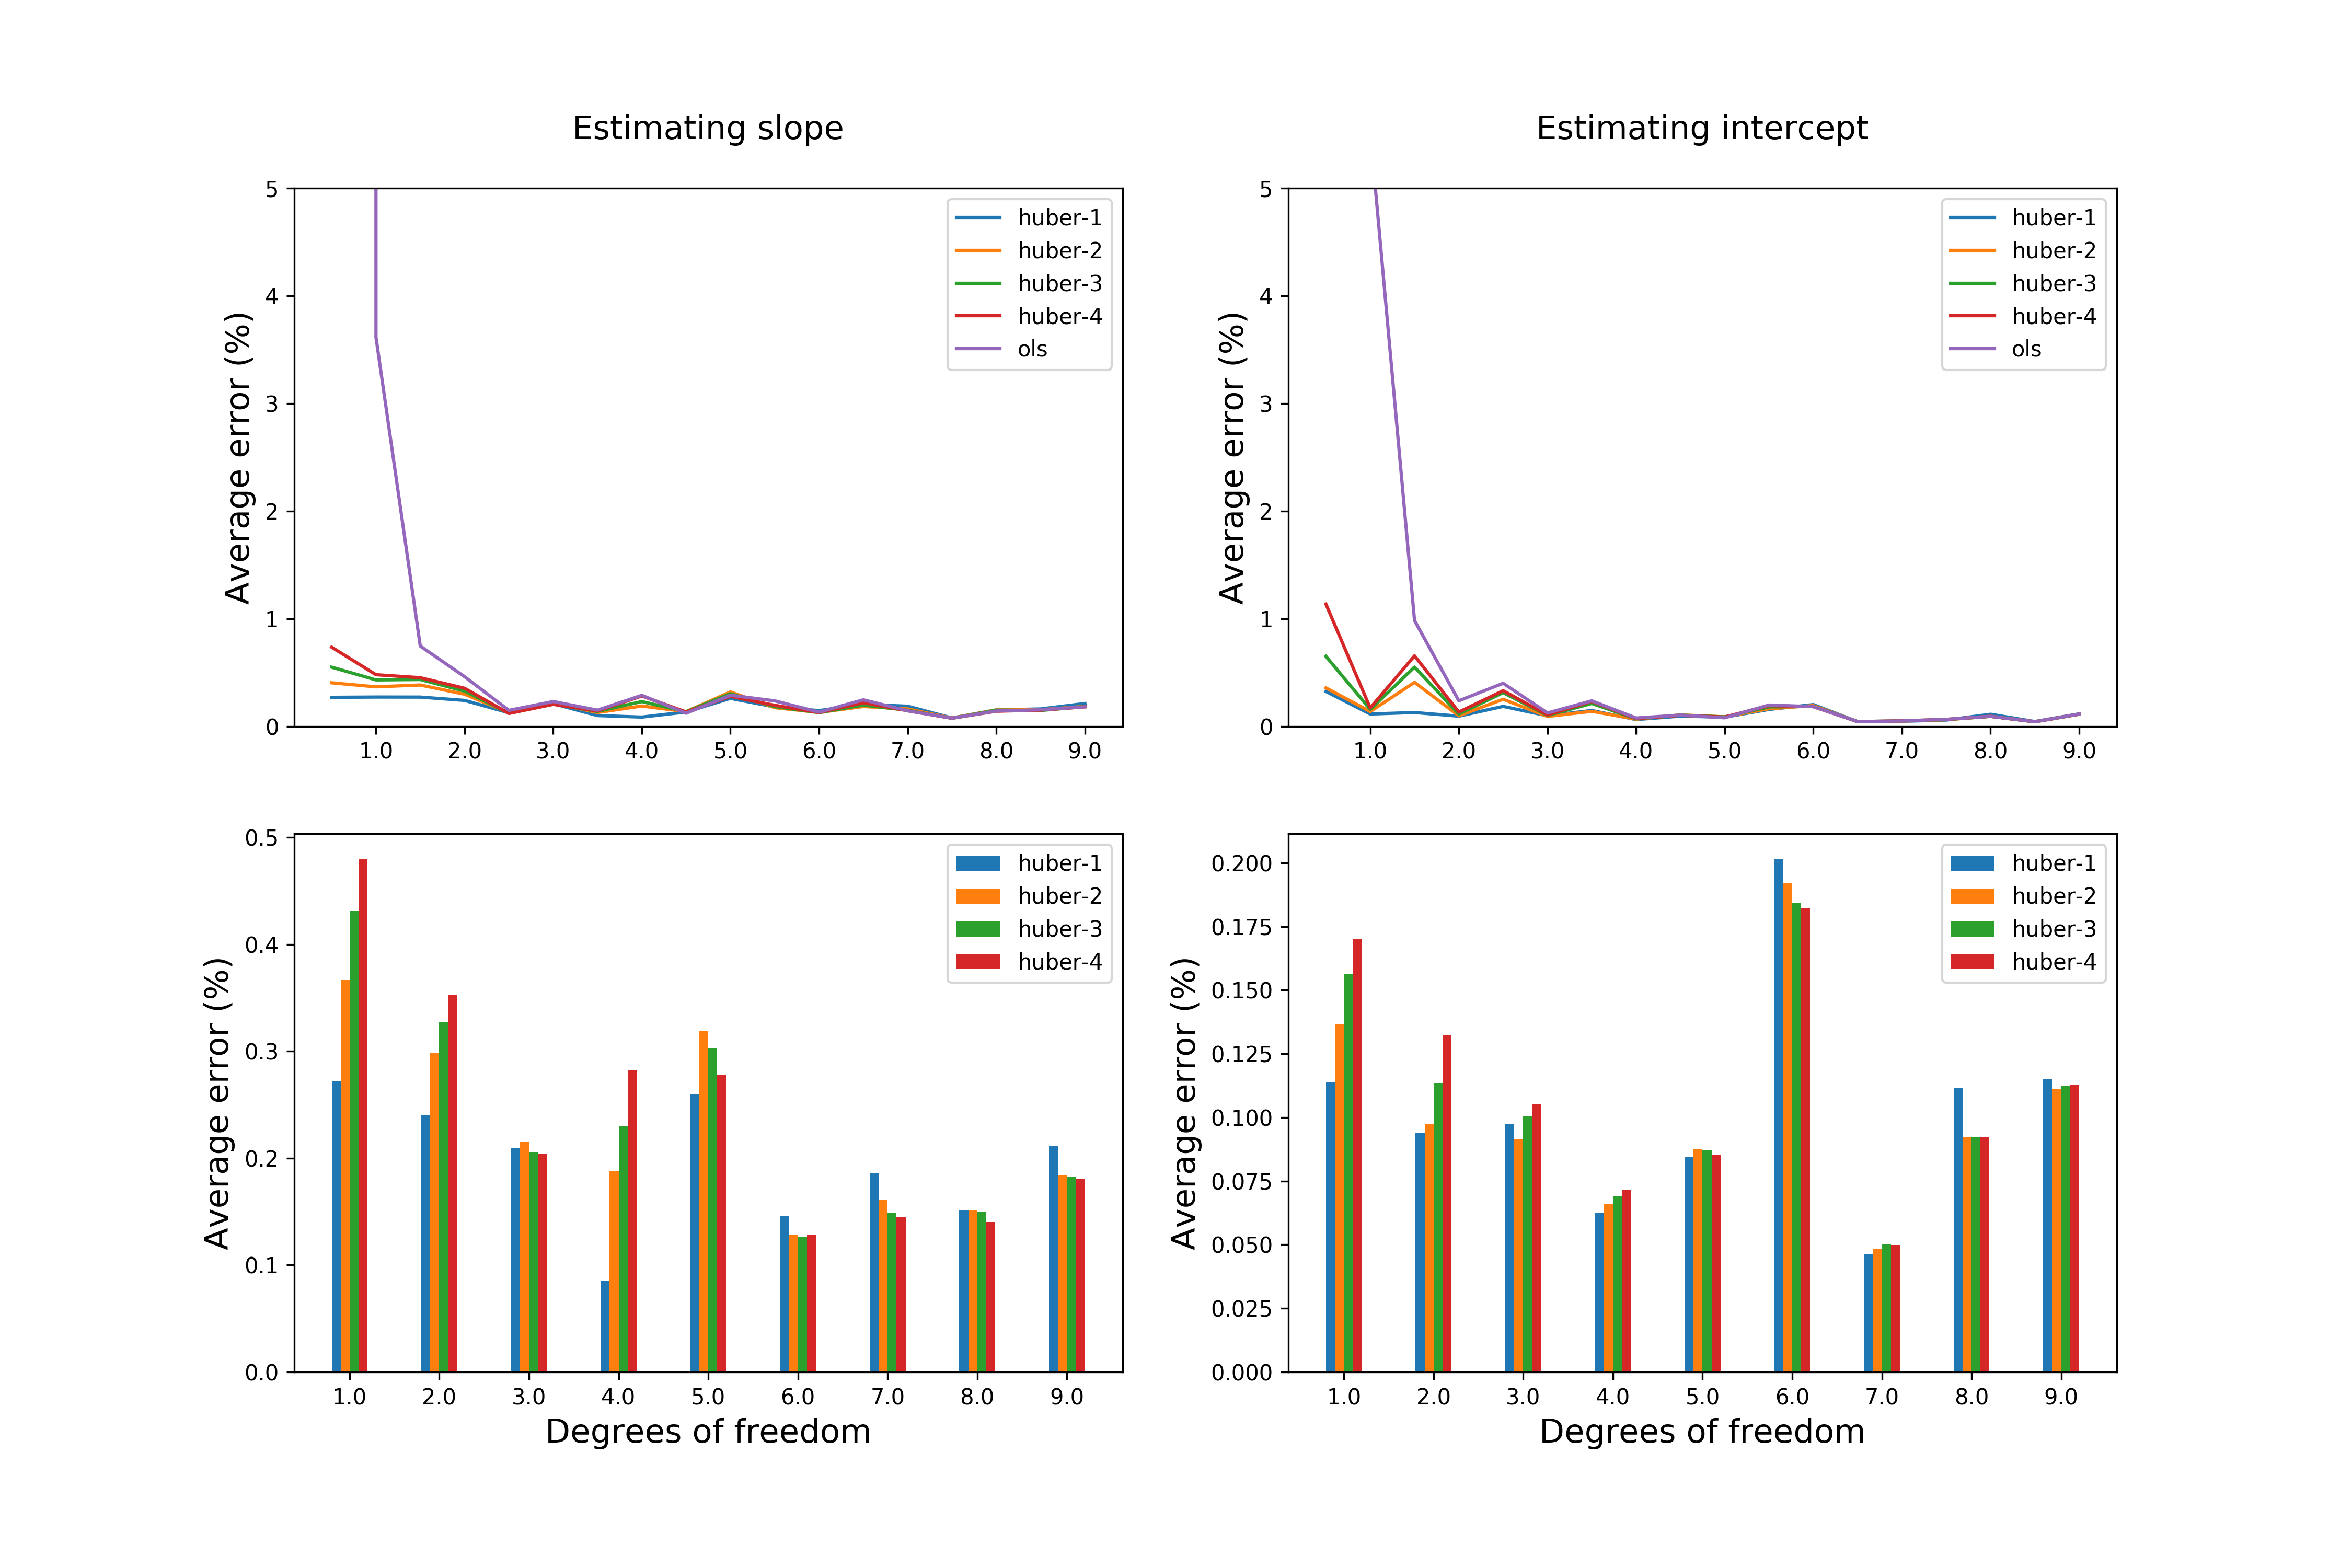
\includegraphics[scale=0.45]{experiment-m.png}
\end{center}
\caption{The left hand figures refer to the slope estimate, and the right hand figures to the intercept estimate. The first row presents an overview including the OLS estimate. The bottom row restricts attention to the Huber estimates for tuning parameters $t=1, 2, 3, 4$.}
\end{figure}

\newpage
\paragraph{Experiment 2.} Comparing the ECME algorithm against the M-estimates.\\

We compare the ECME algorithm's estimates against the M-estimates corresponding to Huber norm $\rho(e; t)$ with tuning parameter $t=1,4$. We see that for small $\nu$ the ECME estimate outperforms the M-estimates.

\begin{figure}[H]
\begin{center}
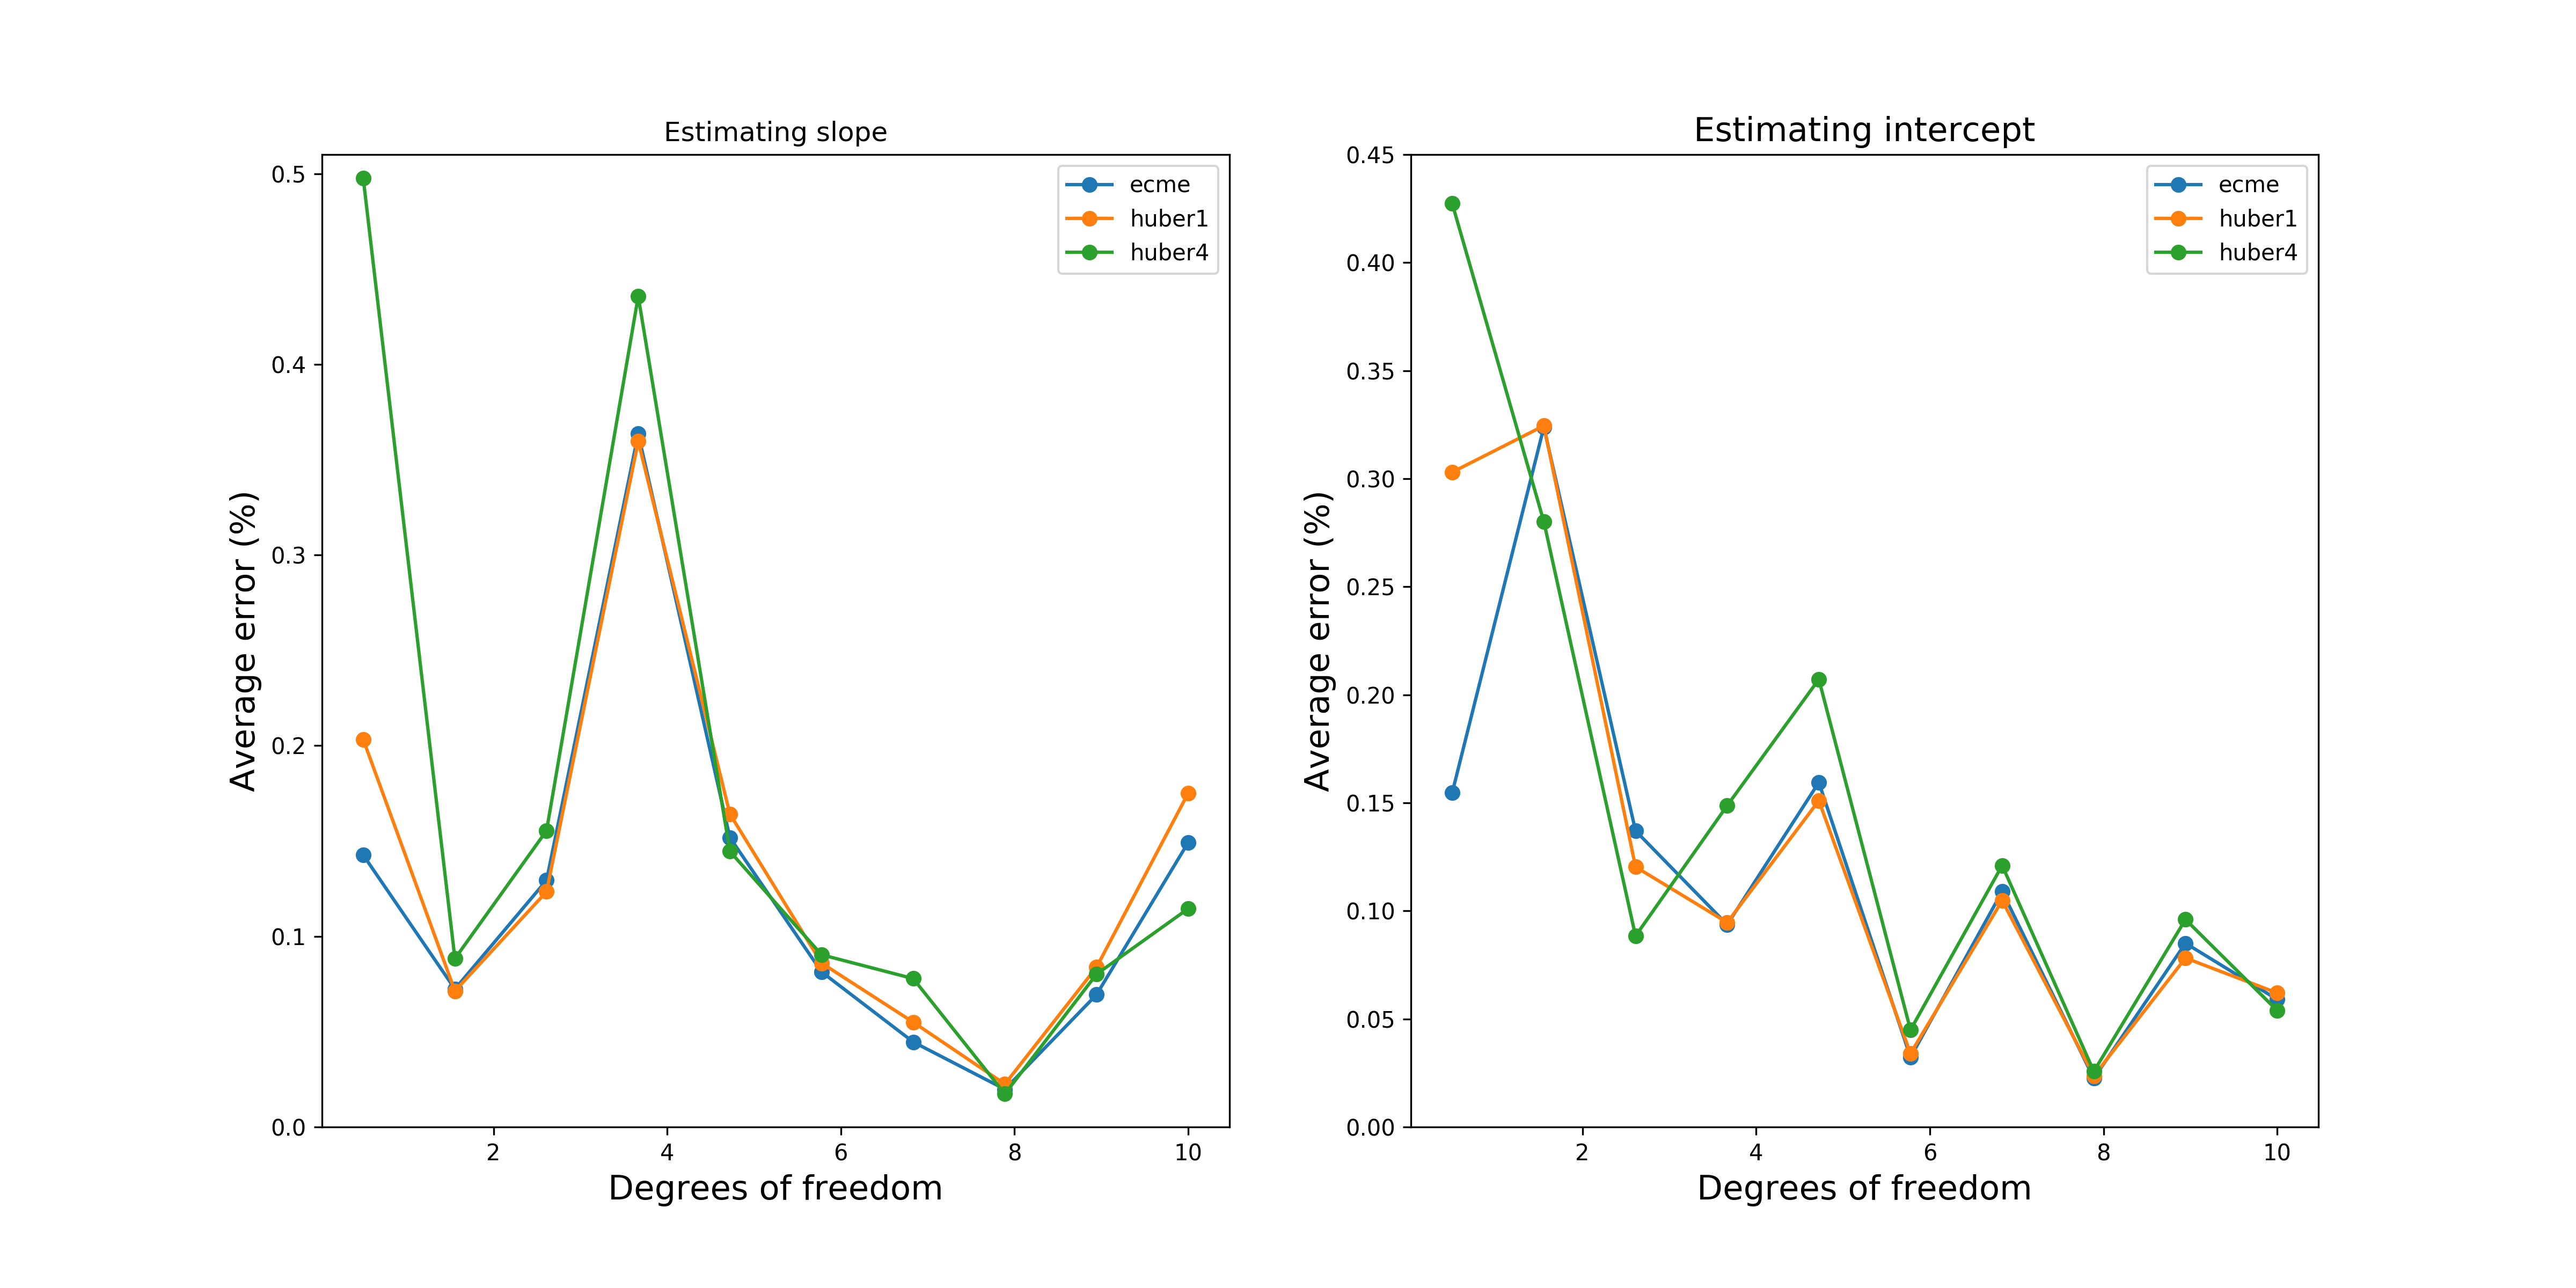
\includegraphics[scale=0.45]{experiment-ecme.png}
\end{center}
\caption{Comparison of estimates using the ECME algorithm, and Huber M-estimates with tuning parameter $t=1$ and $t=4$.}
\end{figure}


\newpage
\section{Results}
We present a brief summary of the estimates provided for each of the five datasets.

\begin{minipage}{.5\textwidth}
\begin{center}
$\begin{array}{c|cc}
\mbox{Filename} & a & b \\\hline
\mbox{data\_1\_1} & 1.078 & -0.265 \\
\mbox{data\_1\_2} & 1.227 & -0.605 \\
\mbox{data\_1\_3} & -0.605 & 1.101 \\
\mbox{data\_1\_4} & 1.422 & 0.130 \\
\mbox{data\_1\_5} & -0.994 & -0.044
\end{array}$
\end{center}
\end{minipage}%
\begin{minipage}{.5\textwidth}
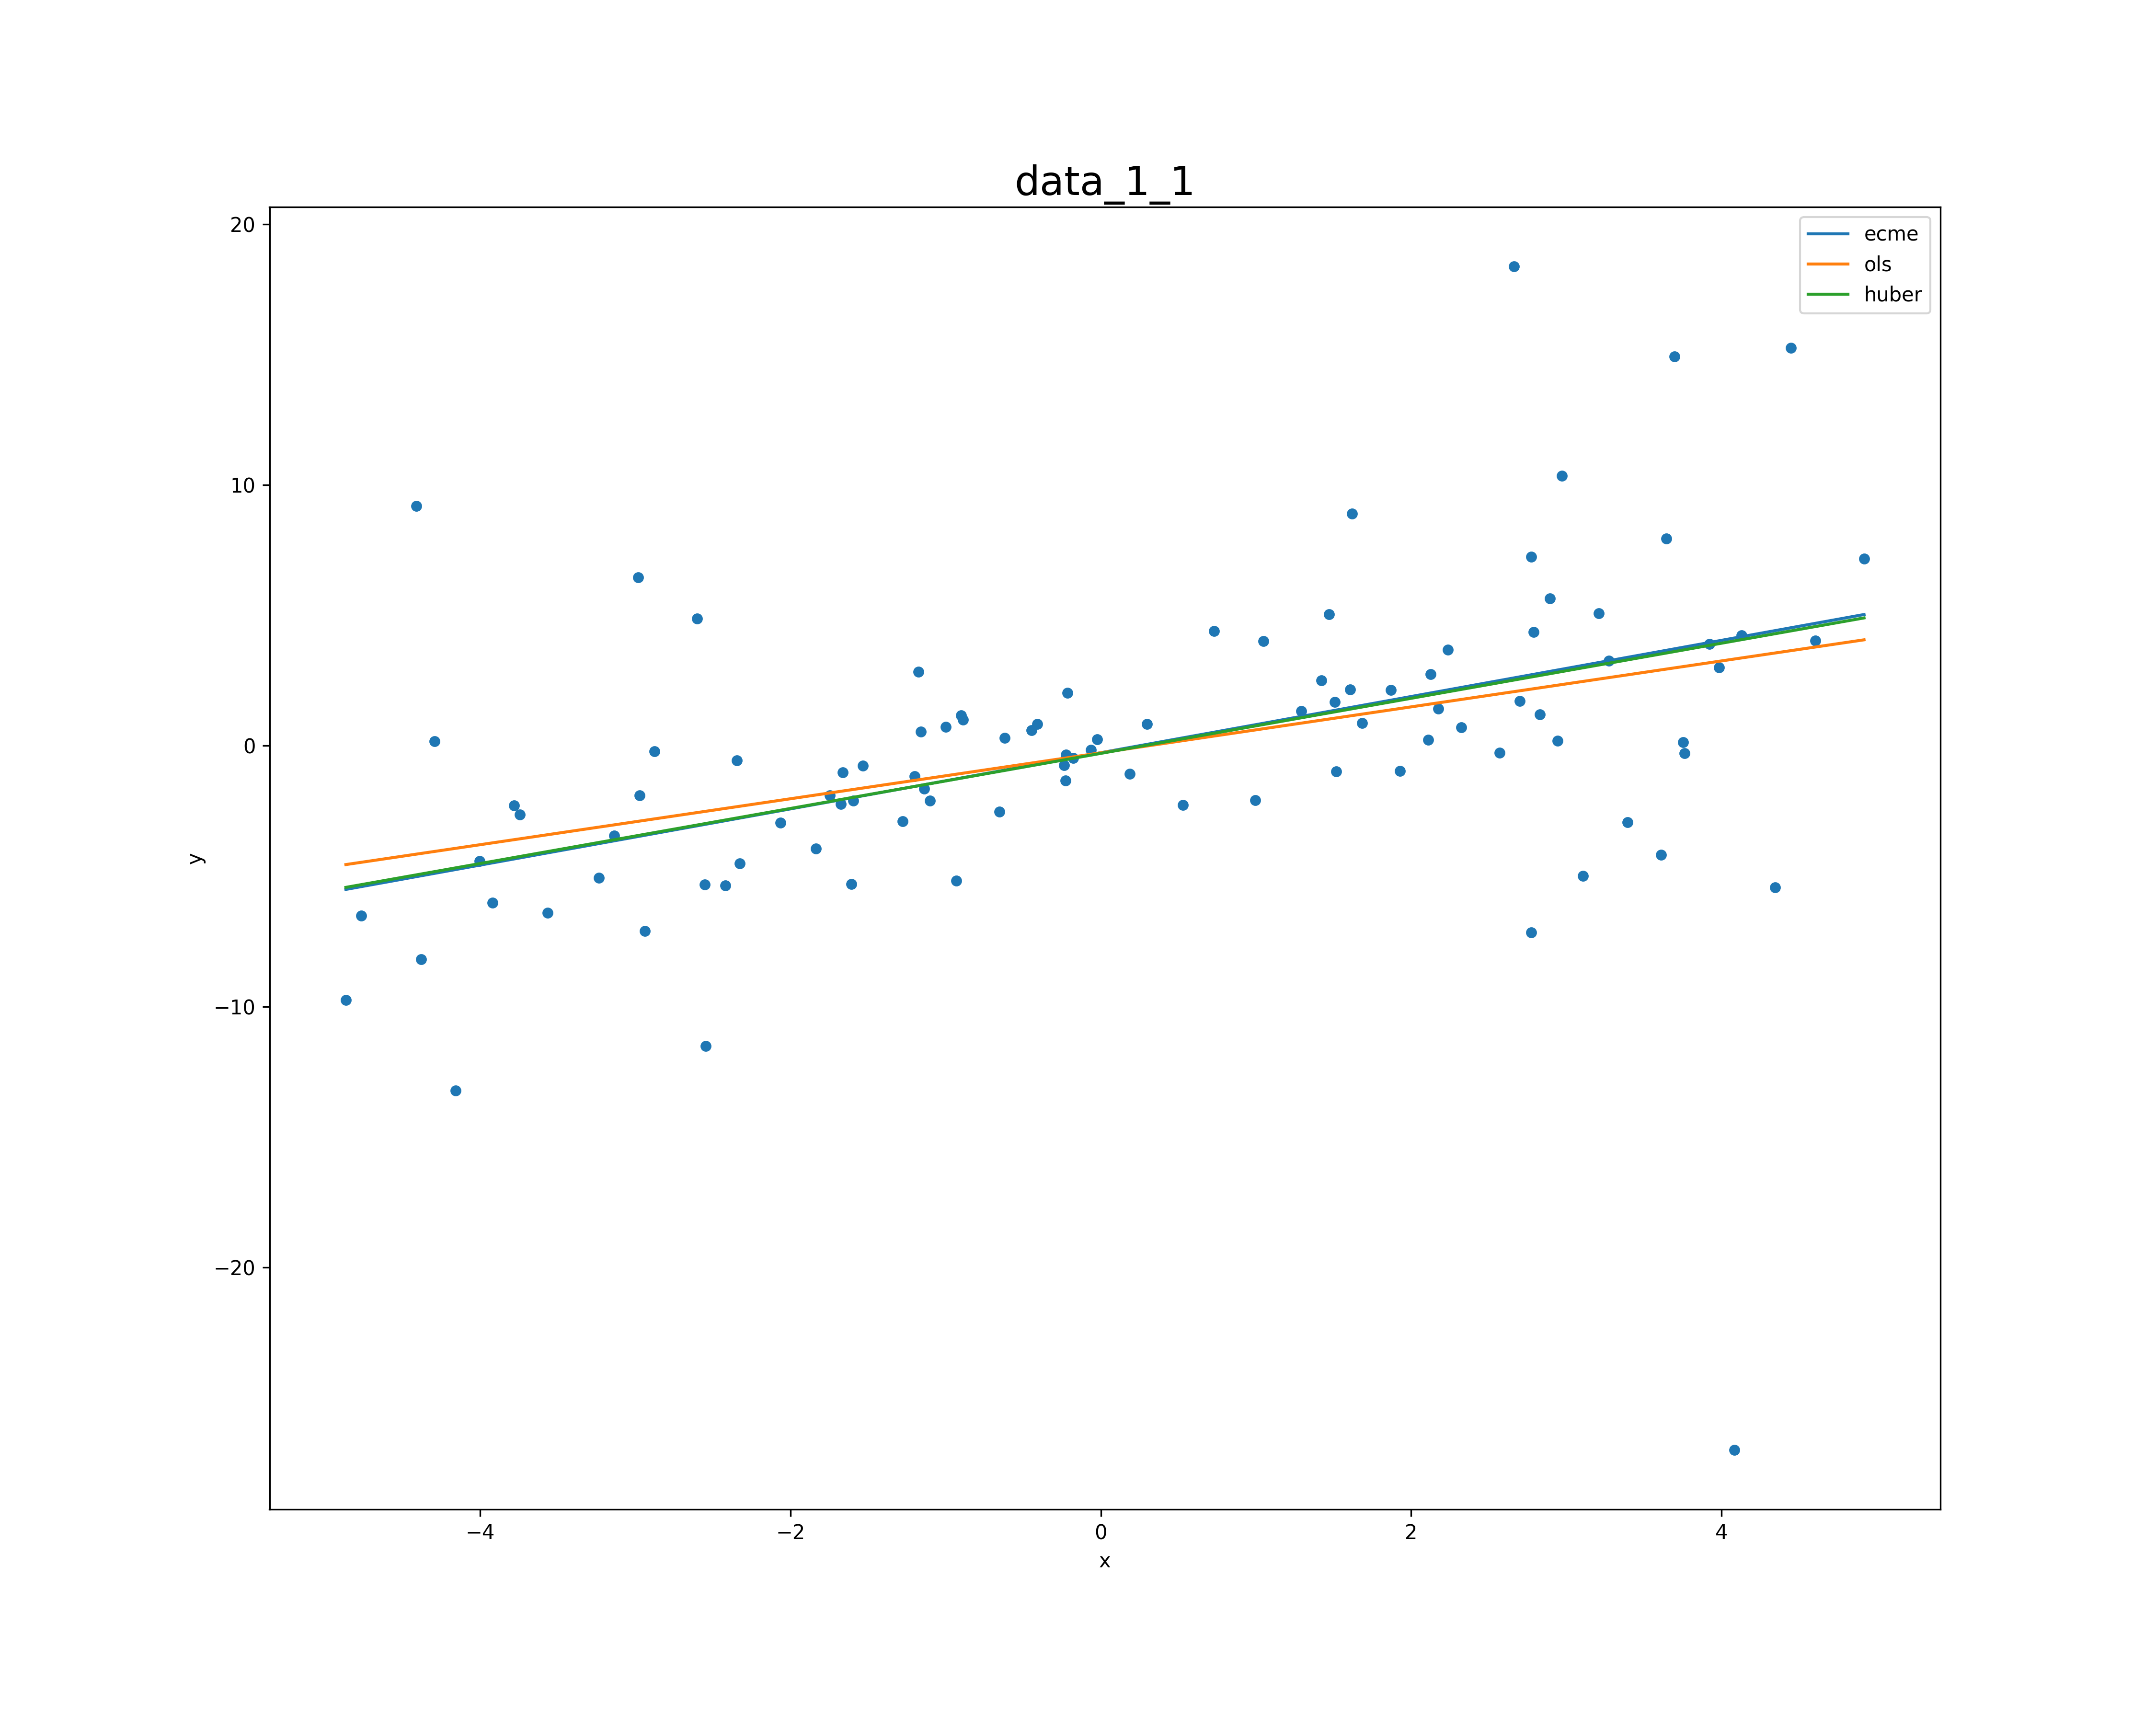
\includegraphics[scale=0.25]{data_1_1-figure.png}
\end{minipage}

\begin{minipage}{.5\textwidth}
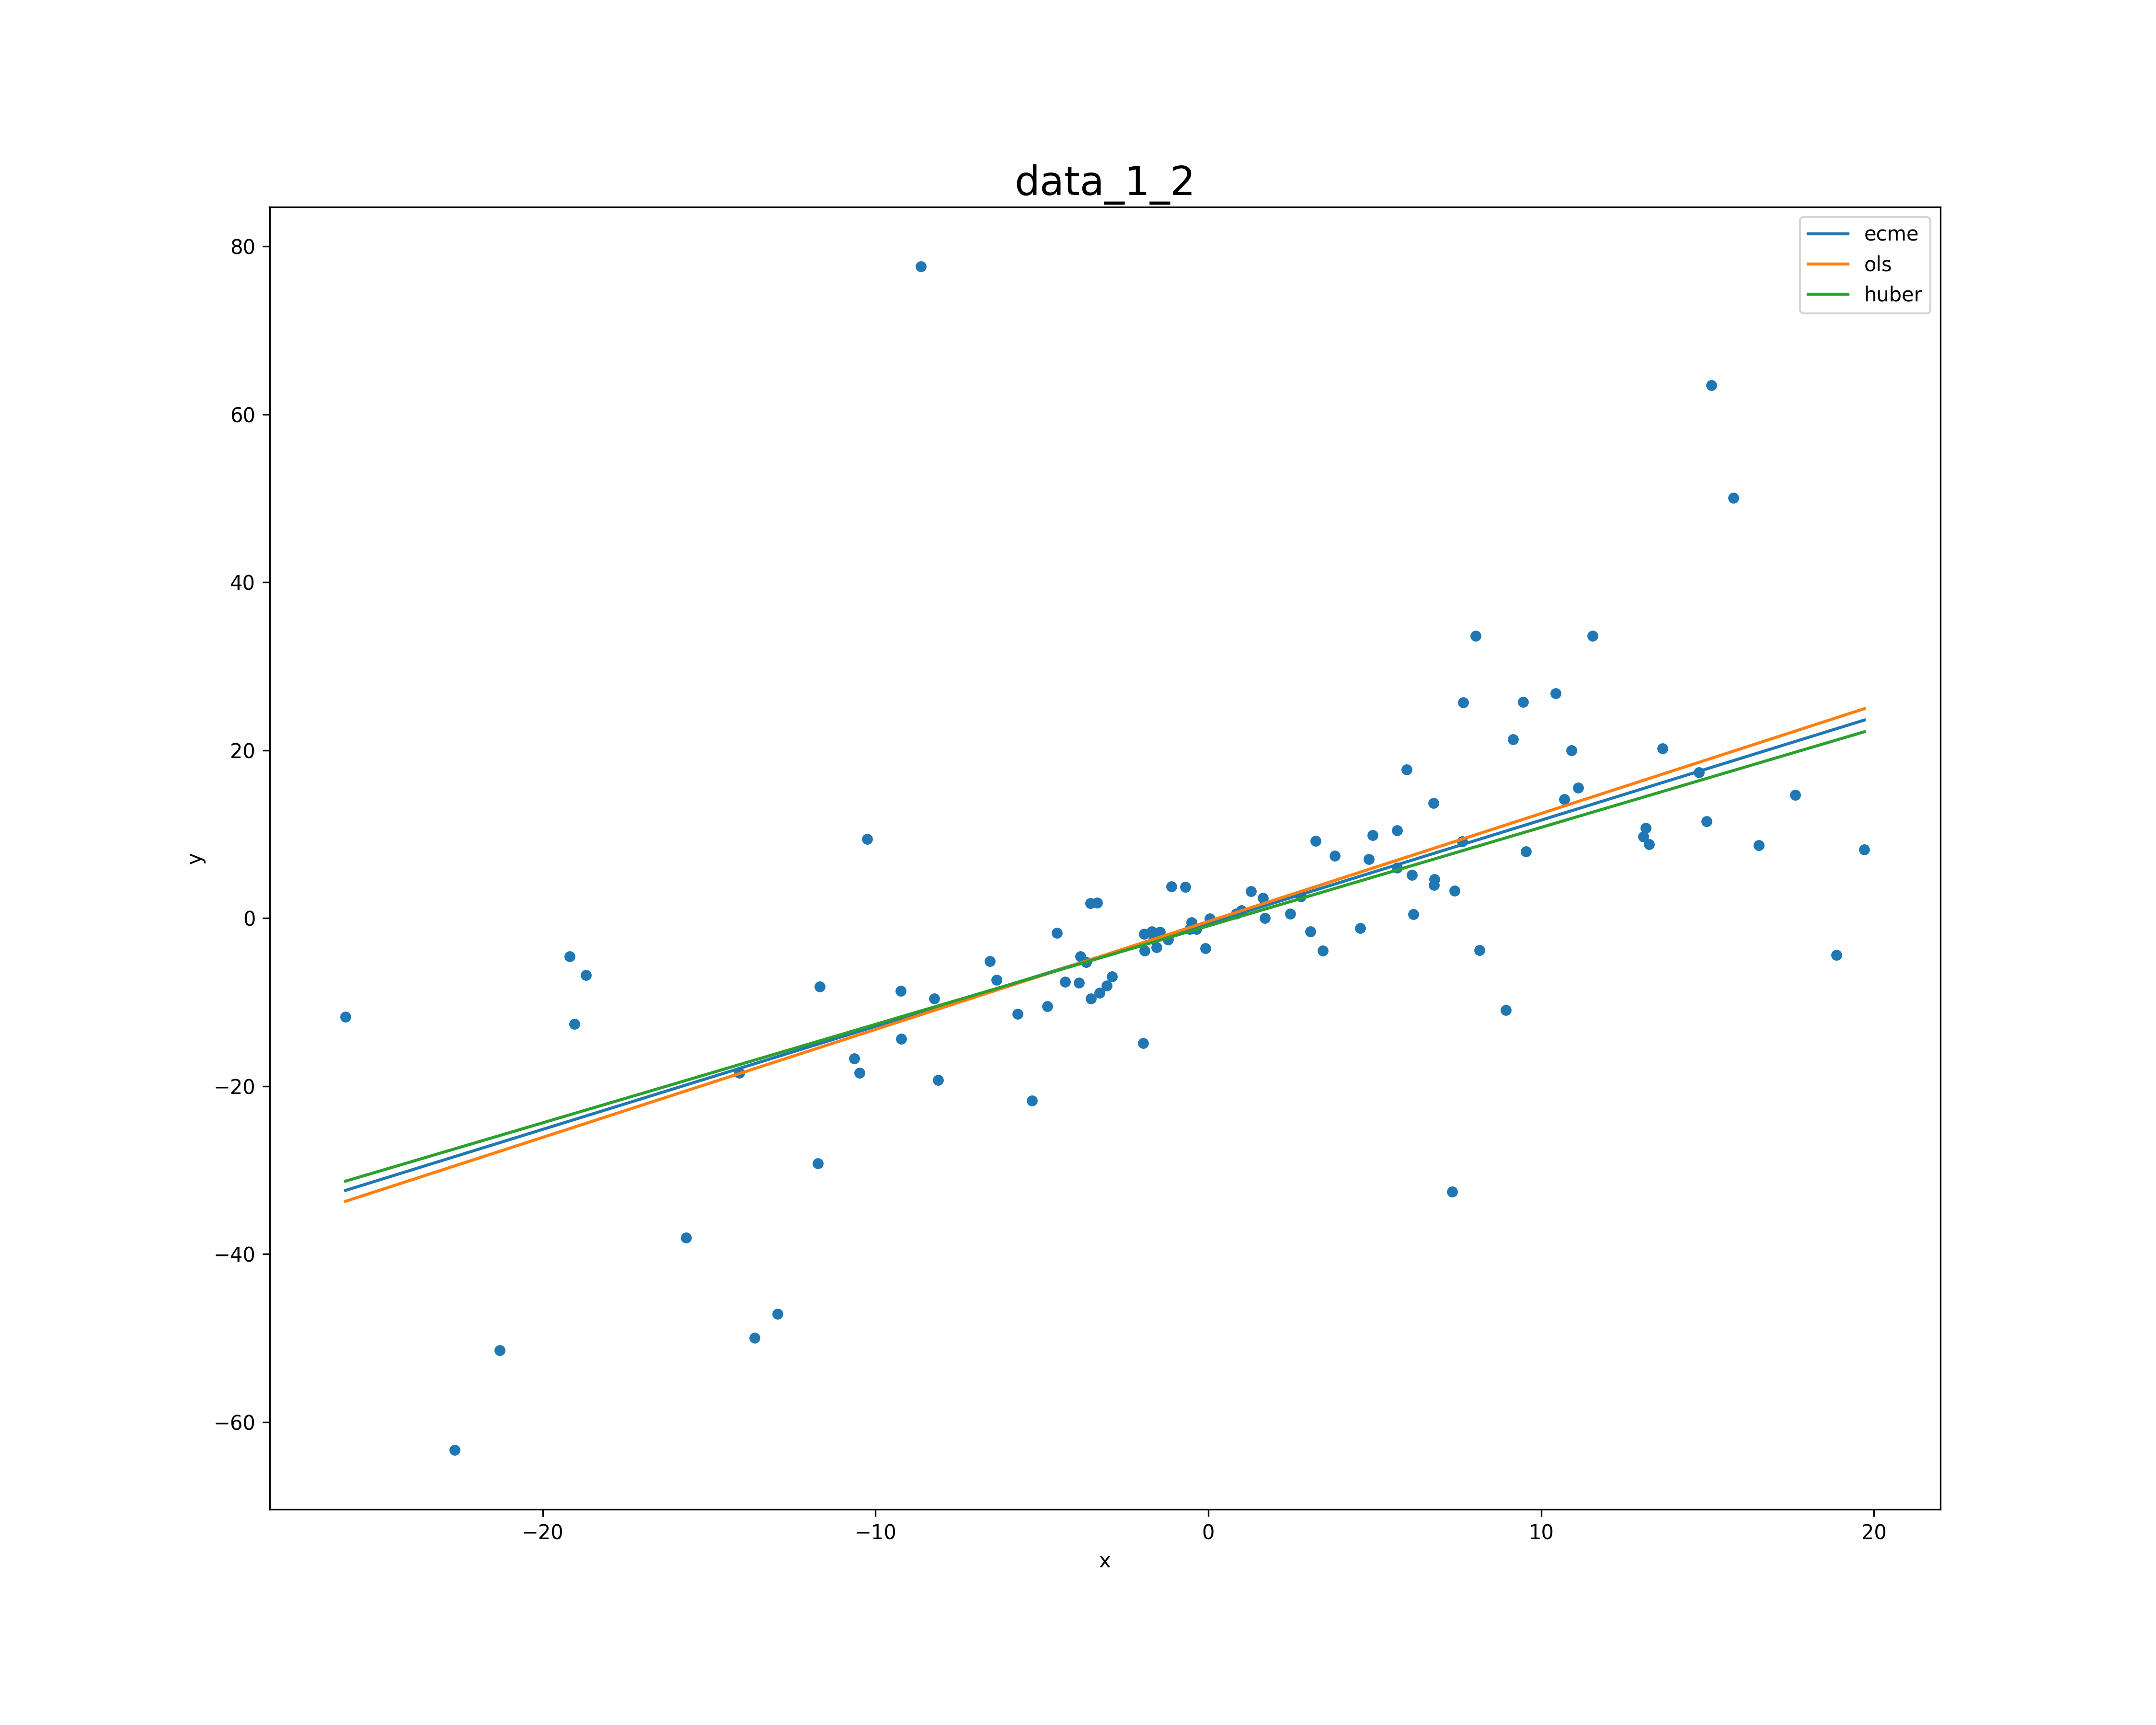
\includegraphics[scale=0.25]{data_1_2-figure.png}
\end{minipage}%
\begin{minipage}{.5\textwidth}
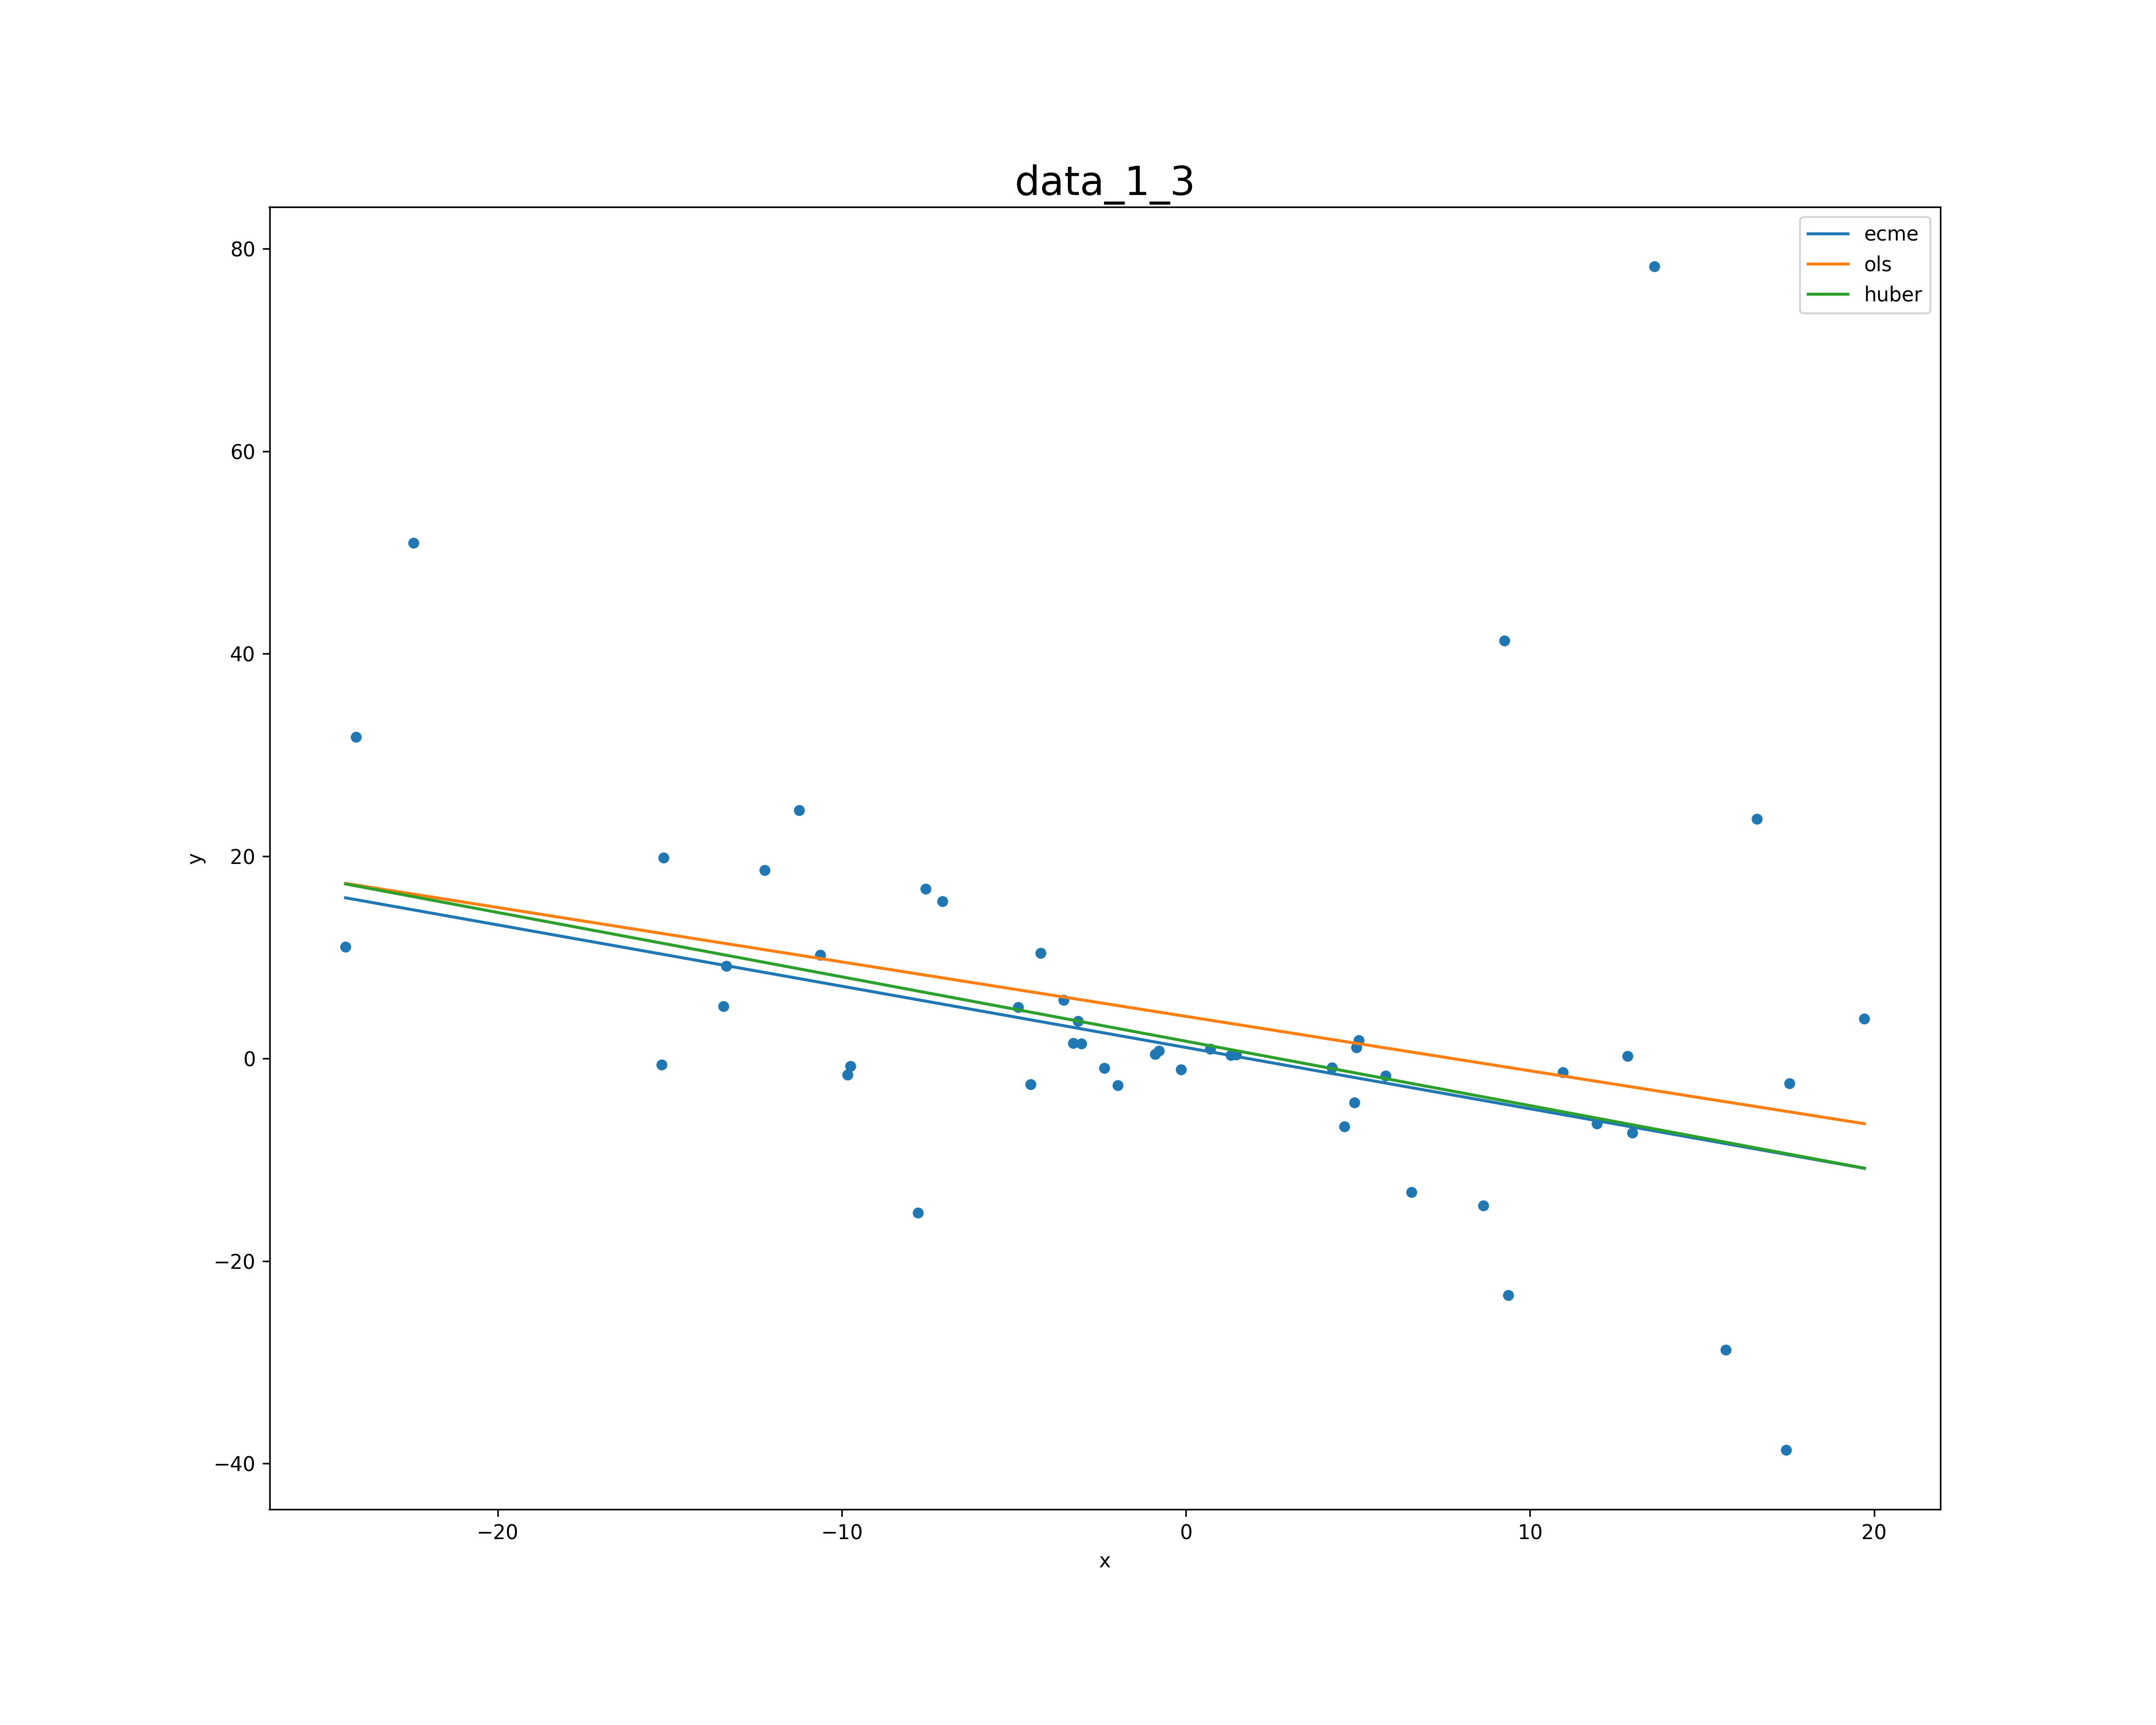
\includegraphics[scale=0.25]{data_1_3-figure.png}
\end{minipage}

\begin{minipage}{.5\textwidth}
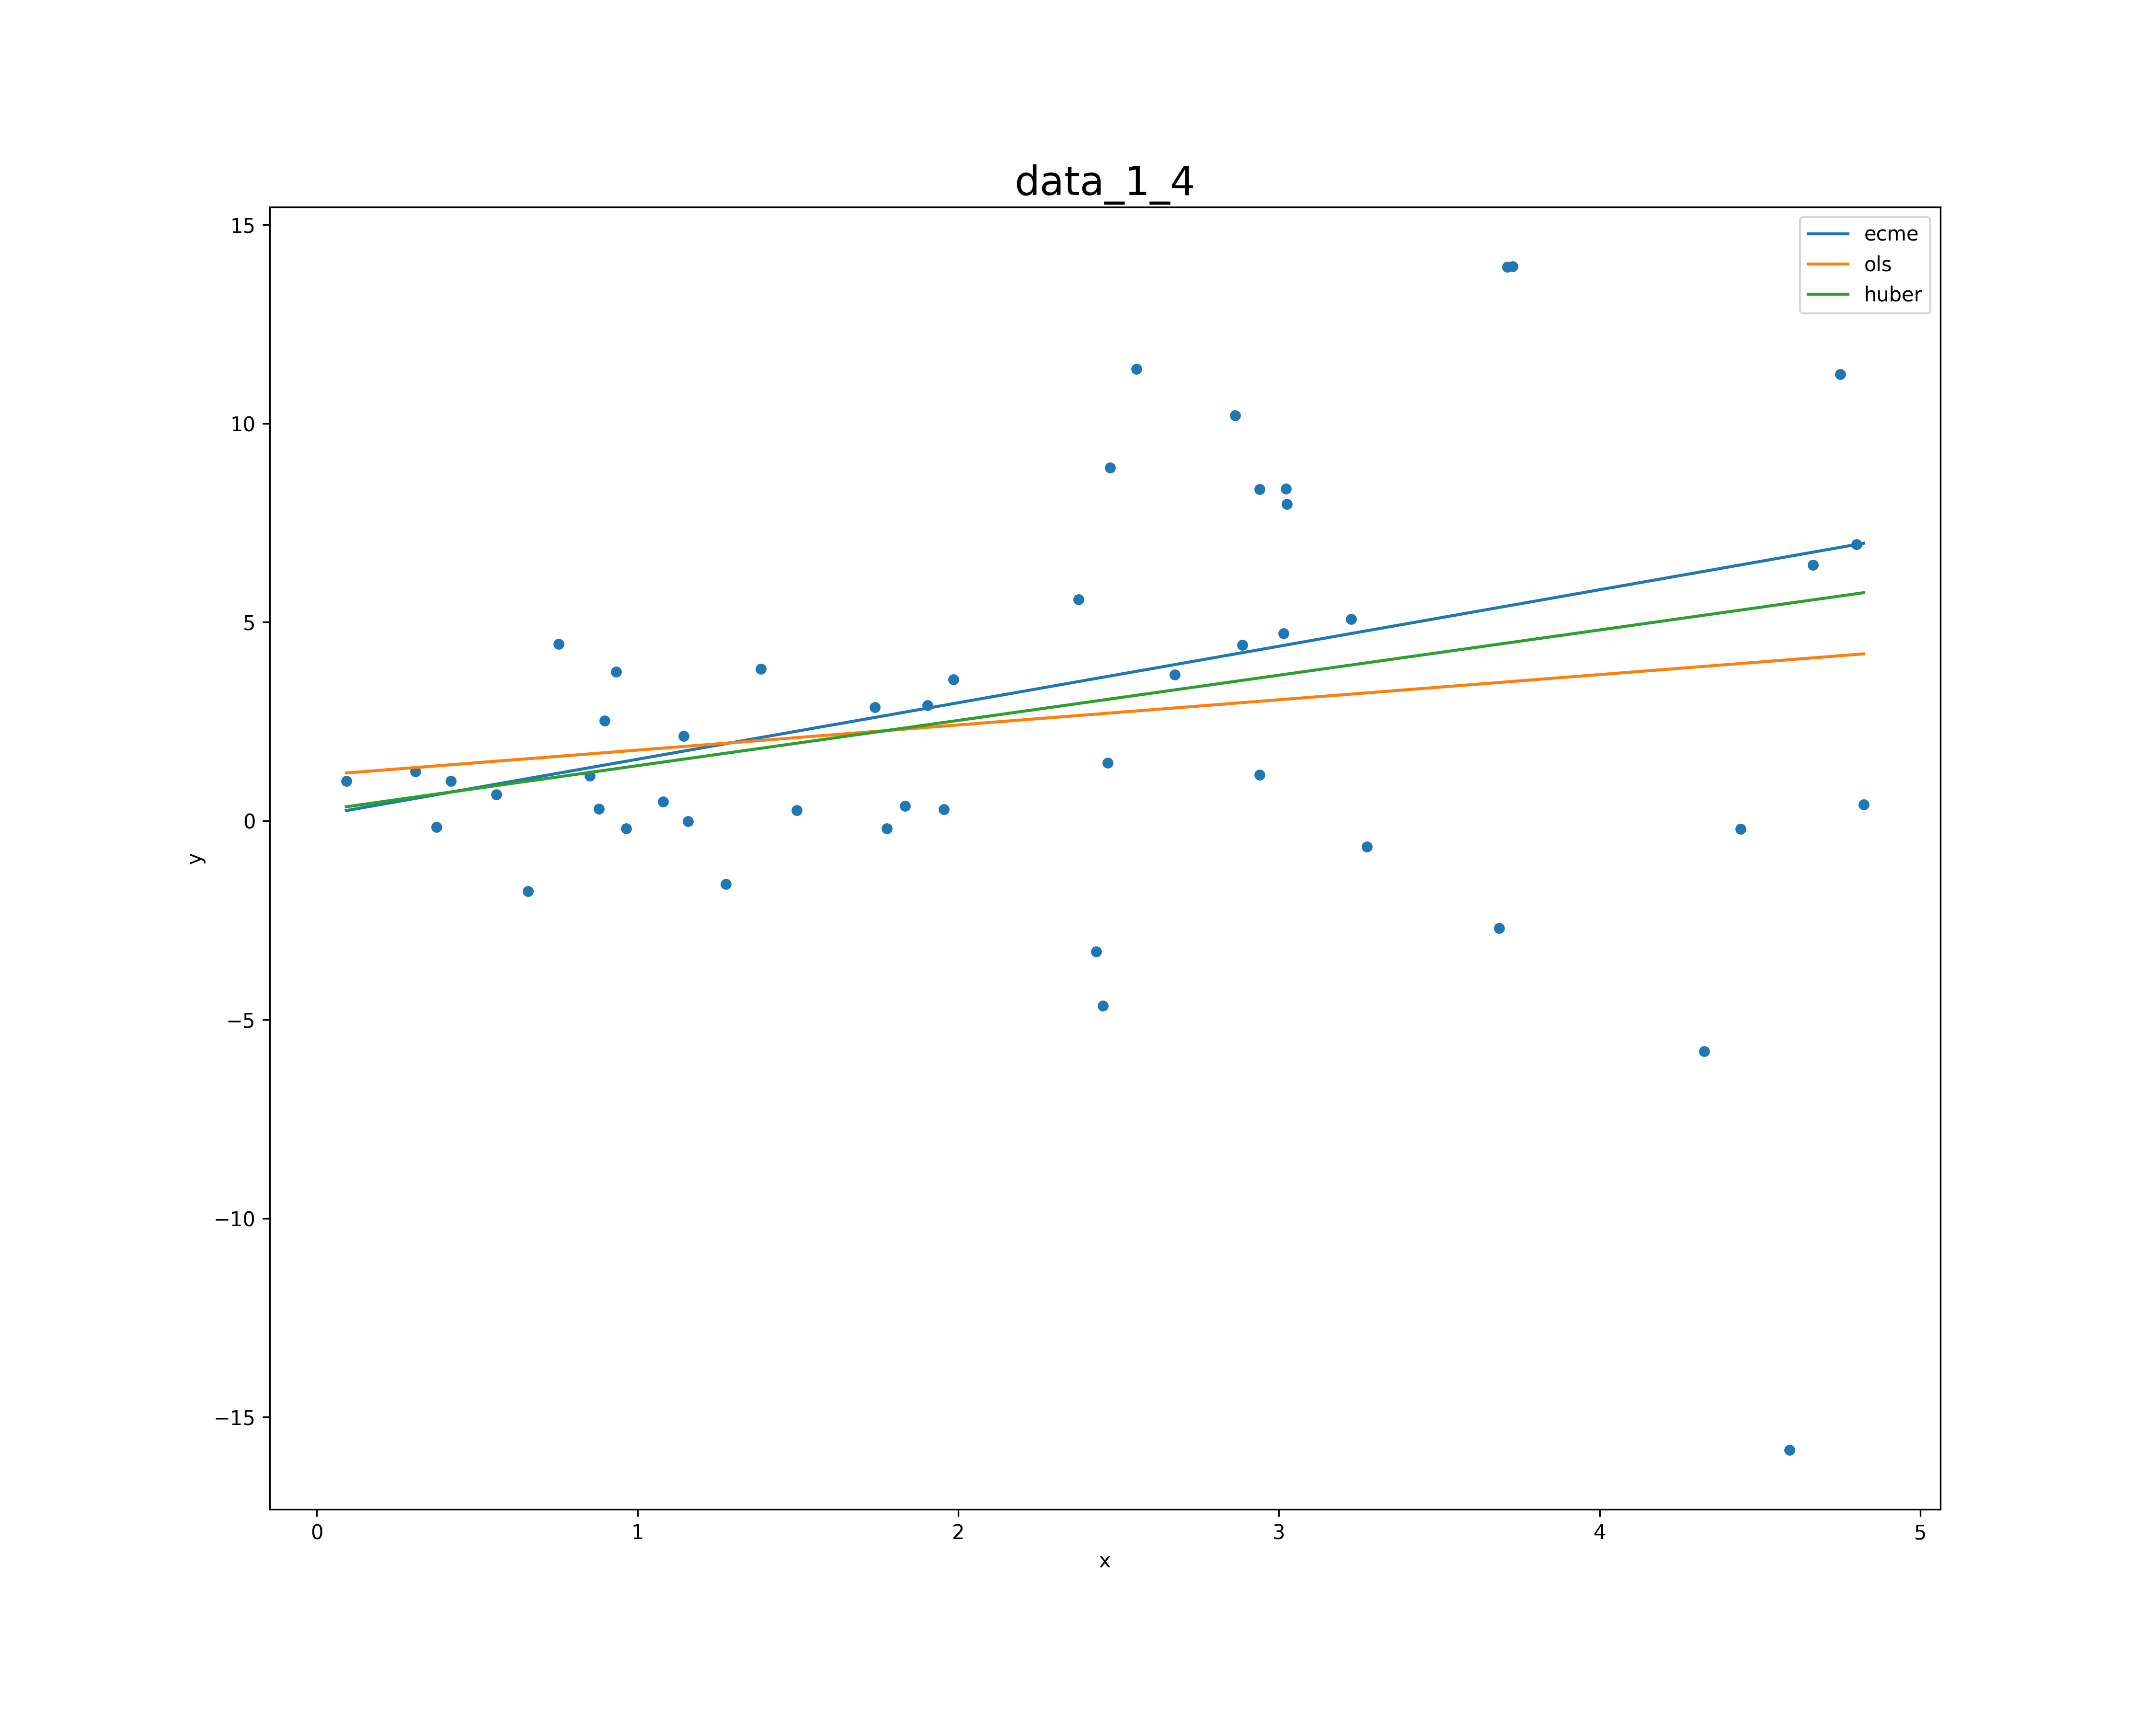
\includegraphics[scale=0.25]{data_1_4-figure.png}
\end{minipage}%
\begin{minipage}{.5\textwidth}
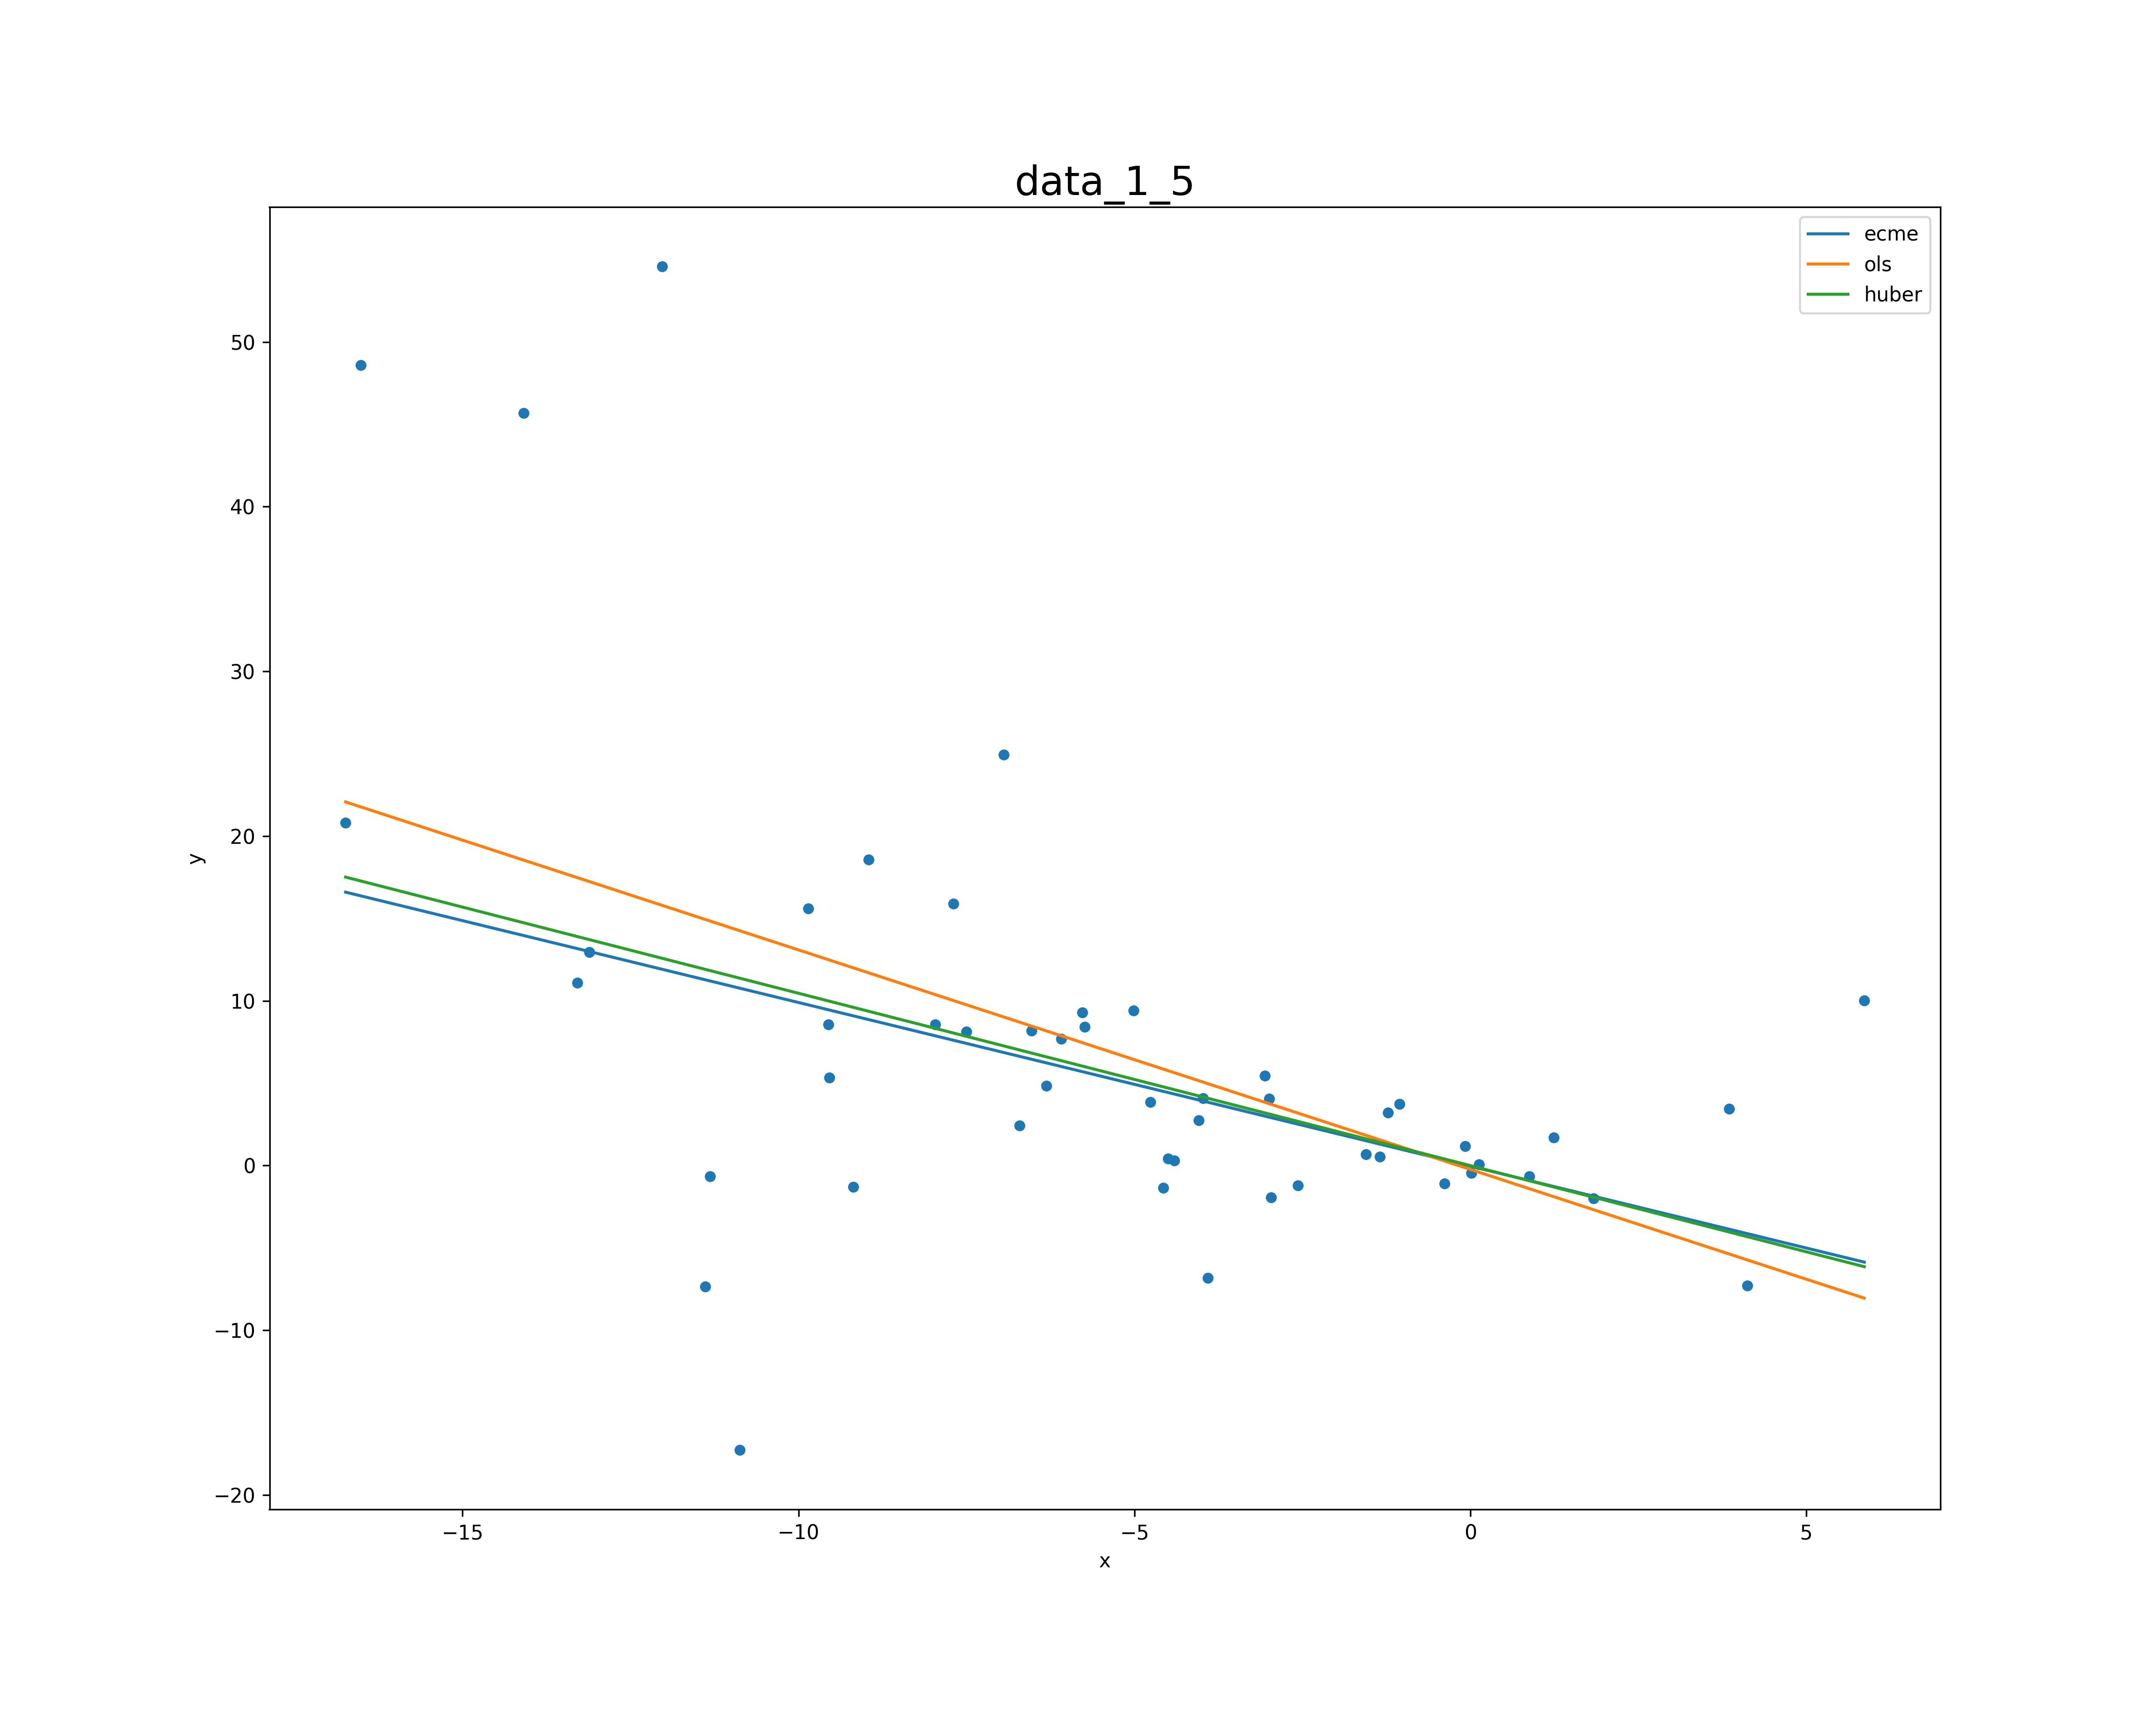
\includegraphics[scale=0.25]{data_1_5-figure.png}
\end{minipage}


\section*{Appendix}
\appendix
\section{M-estimates} \label{SecMest}
Define a \textbf{cost function} $J_\rho$  in terms of an abstract norm $\rho: \mathbb{R} \rightarrow \mathbb{R}$ as,
\[
J_\rho(a,b) = \sum_{i = 1}^N \rho(e_i),
\]
For example, given the function $\rho(e) = \frac{1}{2}{e^2}$, minimizing the cost function $J_\rho(a,b)$ is equivalent to finding the ordinary least squares estimate. We will focus our attention on the Huber norm,
\begin{equation} \label{EqHuber}
\rho(e; t) = \left\{\begin{array}{ccc}\frac{1}{2}e^2 & ~ & |e| < t \\t|e| - \frac{1}{2}t^2 & ~ & \mbox{else}\end{array}\right. \tag{\ref{SecMest}1}
\end{equation}



where $t\in\mathbb{R}_{>0}$ is a tuning parameter. This is a continuous function that assigns quadratic cost to errors of size at most $t$, and otherwise assigns linear cost. Consequently, the associated cost function $J_\rho$ is less sensitive to outliers in the data, as desired.\\


The influence $\psi = \nabla\rho$ is defined as the gradient of $\rho$ with respect to $\Theta = (a,b)$. Notice that minimizing the cost function $J_\rho$ is equivalent to solving the system of equations,
\[
\sum_{i = 1}^N \psi(y_i - B\cdot X_i)X_i = 0.
\]
where we encode $x_i$ as a vector $X_i = (1, x_i)$, and our parameters $(a,b)$ as a vector $B = (b, a)$. By defining the define the \textbf{weight function},
\[
w(e) = \frac{\psi(e)}{e},
\]
we can rewrite this as,
\begin{equation}
\sum_{i = 1}^N w_i(y_i - B\cdot X_i)X_i = 0. \notag
\end{equation}
where $w_i:= w(e_i)$ denotes the weight associated to the $i$-th error. Notice that for the OLS estimate we have that $w(e) = 1$, and it is in this way that the more general class of M-estimates can be seen as a re-weighted least-squares estimate.

\paragraph{Optimization.} It remains to minimize our objective function $J_\rho$. Let $B^{(0)}$ be an initial estimate for the parameter $B$. For example, let $B^{(0)}$ be the usual least squares estimate.\\

Repeat the following until convergence:
\begin{enumerate}

\item Let $e_i^{(t)}$ denote the residuals computed using the estimate $B^{(t)}$.

\item Compute the weights $w_i^{(t)}$ from the residuals $e_i^{(t)}$ via the weight function $w$.

\item Let $B^{(t+1)}$ be the weighted least-squares estimate,
\[
B^{(t+1)} = \argmin \sum_i \left(w_i^{(t+1)} \cdot e_i^{(t+1)}\right)^2.
\]
\end{enumerate}

\paragraph{Implementation.} This algorithm is implemented in the Python library \texttt{statsmodels}.

\section{ECME algorithm} \label{SecECME}
Recall that we have the following equivalent form for our noisy linear model.
\[
y_i | \mu_i, \sigma, w_i \sim \mathcal{N}\left(\mu_i, \sigma^2/w_i\right)
\]
where we write $\mu_i = ax_i + b$ and where,
\[
w_i | \nu \sim \mbox{Gamma}\left(\frac{\nu}{2}, \frac{\nu}{2}\right).
\]
Notice that here the $w_i$'s are playing a similar role to weight function $w$ that arise in the theory of M-estimates in that they serve to detect and down-weight outliers. The advantage of this perspective, however, is that it allows us to employ an EM-type algorithm, which we now describe. This is a modified version of the ECME algorithm of Liu-Rubin \cite{LiuRubin}.\\

Let $y = (y_1, \cdots, y_N)$ and $X = (X_1, \cdots, X_N)$ denote the concatenations of our samples into matrices, each with $N$ rows. Suppose at iteration $t$ you have the following (tentative) estimates $B^{(t)}, w^{(t)}, \sigma^{(t)}, \nu^{(t)}$ for the parameters of interest.

\paragraph{E-step} Set,
\[
w_i^{(t+1)} = \frac{\nu^{(t)} + 1}{\nu^{(t)} + \delta_i^{(t)}},
\]
where $\delta_i^{(t)} = 1/(\sigma^{(t)})^2(y_i - \mu_i^{(t)})$ and $\mu_i^{(t)} = B^{(t)}\cdot X_i$.

\paragraph{CM-step-1}
Set,
\[
B^{(t+1)} = (X'W^{(t)}X)^{-1}X'W^{(t)}y
\]
and
\[
\sigma^{(t+1)} = \sqrt{\frac{\sum_{i=1}^N w_i^{(t+1)}(y_i - \mu_i^{(t+1)})}{N}}
\]

\paragraph{CM-step-2} Find $\nu^{(t+1)}$ as the unique solution in $\mathbb{R}_{>0}$ to
\[
1 - \phi(\nu/2) + \ln(\nu/2) + \frac{\sum_{i=1}^N \ln(w_i) - w_i}{N}  + \frac{\sum_{i=1}^N \phi \left( \frac{\nu+1}{2} \right) - \ln \left( \frac{\nu+1}{2} \right)}{N} = 0
\]
where $\phi(x)$ is the digamma function.

\paragraph{Remarks.}~
\begin{enumerate}
\item It is shown in \cite{LiuRubin} that this algorithm has stable monotone convergence to a local maximum likelihood estimate.
\item In CM-step-2 we use the bisection method to find the solution $\nu^{(t+1)}$.
\end{enumerate}




\bibliography{/Users/Amin/Dropbox/Math/Latex/coreFiles/aminbib}
\bibliographystyle{acm}


%\printindex


\end{document}